% Options for packages loaded elsewhere
\PassOptionsToPackage{unicode}{hyperref}
\PassOptionsToPackage{hyphens}{url}
%
\documentclass[
]{book}
\usepackage{amsmath,amssymb}
\usepackage{iftex}
\ifPDFTeX
  \usepackage[T1]{fontenc}
  \usepackage[utf8]{inputenc}
  \usepackage{textcomp} % provide euro and other symbols
\else % if luatex or xetex
  \usepackage{unicode-math} % this also loads fontspec
  \defaultfontfeatures{Scale=MatchLowercase}
  \defaultfontfeatures[\rmfamily]{Ligatures=TeX,Scale=1}
\fi
\usepackage{lmodern}
\ifPDFTeX\else
  % xetex/luatex font selection
\fi
% Use upquote if available, for straight quotes in verbatim environments
\IfFileExists{upquote.sty}{\usepackage{upquote}}{}
\IfFileExists{microtype.sty}{% use microtype if available
  \usepackage[]{microtype}
  \UseMicrotypeSet[protrusion]{basicmath} % disable protrusion for tt fonts
}{}
\makeatletter
\@ifundefined{KOMAClassName}{% if non-KOMA class
  \IfFileExists{parskip.sty}{%
    \usepackage{parskip}
  }{% else
    \setlength{\parindent}{0pt}
    \setlength{\parskip}{6pt plus 2pt minus 1pt}}
}{% if KOMA class
  \KOMAoptions{parskip=half}}
\makeatother
\usepackage{xcolor}
\usepackage{longtable,booktabs,array}
\usepackage{calc} % for calculating minipage widths
% Correct order of tables after \paragraph or \subparagraph
\usepackage{etoolbox}
\makeatletter
\patchcmd\longtable{\par}{\if@noskipsec\mbox{}\fi\par}{}{}
\makeatother
% Allow footnotes in longtable head/foot
\IfFileExists{footnotehyper.sty}{\usepackage{footnotehyper}}{\usepackage{footnote}}
\makesavenoteenv{longtable}
\usepackage{graphicx}
\makeatletter
\def\maxwidth{\ifdim\Gin@nat@width>\linewidth\linewidth\else\Gin@nat@width\fi}
\def\maxheight{\ifdim\Gin@nat@height>\textheight\textheight\else\Gin@nat@height\fi}
\makeatother
% Scale images if necessary, so that they will not overflow the page
% margins by default, and it is still possible to overwrite the defaults
% using explicit options in \includegraphics[width, height, ...]{}
\setkeys{Gin}{width=\maxwidth,height=\maxheight,keepaspectratio}
% Set default figure placement to htbp
\makeatletter
\def\fps@figure{htbp}
\makeatother
\setlength{\emergencystretch}{3em} % prevent overfull lines
\providecommand{\tightlist}{%
  \setlength{\itemsep}{0pt}\setlength{\parskip}{0pt}}
\setcounter{secnumdepth}{5}
\usepackage{booktabs}
\ifLuaTeX
  \usepackage{selnolig}  % disable illegal ligatures
\fi
\usepackage{bookmark}
\IfFileExists{xurl.sty}{\usepackage{xurl}}{} % add URL line breaks if available
\urlstyle{same}
\hypersetup{
  hidelinks,
  pdfcreator={LaTeX via pandoc}}

\author{}
\date{\vspace{-2.5em}}

\begin{document}

{
\setcounter{tocdepth}{1}
\tableofcontents
}
\chapter*{}\label{section}
\addcontentsline{toc}{chapter}{}

\chapter{Introduction générale}\label{introduction-guxe9nuxe9rale}

Les enchères constituent un mécanisme central d'allocation des ressources en économie. De manière générale, une enchère peut être définie comme une procédure de vente par laquelle un ou plusieurs biens sont attribués à des acheteurs potentiels, appelés \emph{enchérisseurs}, sur la base d'offres exprimant le prix qu'ils sont prêts à payer. L'attribution du bien, ainsi que le paiement effectif, dépendent de règles précises qui définissent le format de l'enchère. Ces mécanismes sont utilisés dans des contextes variés, allant des marchés traditionnels --- tels que la vente d'œuvres d'art, de biens immobiliers ou de vins rares --- à des environnements économiques contemporains à forte intensité stratégique, comme l'attribution de licences de télécommunications, les marchés de l'électricité ou la publicité en ligne.

L'intérêt analytique des enchères réside dans le fait qu'elles mettent en interaction des agents \emph{rationnels} poursuivant des \emph{objectifs individuels}, tout en disposant d'une \emph{information imparfaite}. Chaque enchérisseur cherche à maximiser son gain, généralement défini comme la différence entre la valeur qu'il attribue au bien et le prix effectivement payé, tout en tenant compte à la fois des règles de l'enchère et du comportement anticipé des autres participants. Cette combinaison d'interactions stratégiques et d'asymétrie d'information fait des enchères un objet central de la théorie des jeux.

La littérature économique distingue classiquement les enchères selon plusieurs dimensions.

\begin{itemize}
\item
  Une première dimension concerne le \emph{nombre de biens mis en vente} : certaines enchères portent sur un bien unique, tandis que d'autres concernent plusieurs biens.
\item
  Une deuxième dimension est la \emph{règle de paiement}. Dans une enchère au premier prix, le gagnant paie le montant exact de son offre, tandis que, dans une enchère au second prix --- également appelée enchère de Vickrey --- le gagnant est celui qui a soumis l'offre la plus élevée, mais il ne paie que la seconde offre la plus élevée.
\item
  Une troisième dimension est la \emph{structure de l'information}. Dans les enchères à valeurs privées, chaque enchérisseur connaît sa propre valorisation du bien, mais ignore celles des autres participants. À l'inverse, dans les enchères à valeurs communes, la valeur réelle du bien est identique pour tous, mais elle est incertaine au moment de l'enchère et les enchérisseurs ne disposent que de signaux imparfaits à son sujet.
\item
  Enfin, les enchères se distinguent par le \emph{mode de soumission des offres}. Dans les enchères simultanées, les enchérisseurs soumettent leurs offres en même temps, sans observer celles des autres. Dans les enchères séquentielles, en revanche, les décisions sont prises dans le temps et les actions passées --- offres, retraits ou annonces de prix --- sont observables et peuvent influencer les décisions futures.
\end{itemize}

C'est dans ce cadre général que s'inscrit la notion d'\textbf{enchère séquentielle}. Toutefois, la littérature ne propose pas une définition unique de la séquentialité. Selon les sources et les contextes étudiés, celle-ci peut être appréhendée suivant \textbf{deux angles distincts}.

Un premier angle, largement adopté dans les travaux consacrés aux enchères multi-objets (Milgrom, 2004 ; Krishna, 2010), définit la séquentialité par le \emph{nombre et l'ordre de mise en vente des biens}. Une enchère est alors dite séquentielle lorsque plusieurs biens sont vendus l'un après l'autre, chaque vente constituant une étape d'un processus intertemporel. Dans ce cadre, les enchérisseurs tiennent compte non seulement de leur valorisation immédiate du bien courant, mais également des opportunités futures, des contraintes budgétaires éventuelles et de l'information révélée par les prix et les résultats des enchères précédentes.

Un second angle, issu d'une approche plus générale de la théorie des jeux dynamiques --- notamment chez Aliprantis, Chakrabarti et Miller ---, définit la séquentialité par la \emph{structure temporelle de la procédure de décision elle-même}, indépendamment du nombre de biens mis en vente. Selon cette perspective, une enchère peut être qualifiée de séquentielle même lorsqu'un seul bien est en jeu, dès lors que les décisions des agents sont prises successivement et que les actions passées sont observables. Les enchères orales, les enchères ascendantes ou certains mécanismes à prix annoncé illustrent cette conception procédurale de la séquentialité. C'est cette conception que nous privilégierons pour la suite de ce travail.

L'analyse des enchères séquentielles met en évidence trois mécanismes centraux.

\begin{itemize}
\tightlist
\item
  Tout d'abord, \textbf{l'apprentissage}, par lequel les enchérisseurs mettent à jour leurs croyances à partir des actions observées au cours du jeu.\\
\item
  Ensuite, \textbf{l'anticipation}, qui conduit les agents à intégrer les conséquences futures de leurs décisions présentes dans leur calcul stratégique.\\
\item
  Enfin, \textbf{l'interaction stratégique dynamique}, qui se manifeste par des comportements de signalisation, de retenue ou d'agressivité en fonction des croyances et des anticipations mutuelles.
\end{itemize}

Dans ce contexte, une question centrale se pose naturellement : \emph{comment la séquentialité modifie-t-elle les stratégies des enchérisseurs et l'issue de l'enchère ?} L'étude de cette question requiert un cadre analytique capable de prendre en compte à la fois la dynamique temporelle du jeu et l'évolution des croyances face à l'information révélée. C'est précisément le rôle de l'\textbf{équilibre parfait bayésien}, qui constitue le concept de solution central de ce travail.

Afin d'analyser les enchères séquentielles dans le cadre des jeux dynamiques à information incomplète, ce document est organisé comme suit. La première partie présente l'enchère séquentielle comme un jeu dynamique, en mettant en évidence le rôle de la Nature et de l'asymétrie d'information. La deuxième partie étudie la dynamique du jeu et la formation des croyances. La troisième partie est consacrée à la définition et à l'analyse de l'équilibre parfait bayésien. Enfin, une application théorique et numérique illustre concrètement les mécanismes stratégiques induits par la séquentialité.

\chapter{Cadre théorique : l'enchère séquentielle comme jeu dynamique à information incomplète (bien unique)}\label{cadre-thuxe9orique-lenchuxe8re-suxe9quentielle-comme-jeu-dynamique-uxe0-information-incompluxe8te-bien-unique}

Cette section établit le cadre théorique mobilisé pour analyser une enchère séquentielle portant sur un bien unique.\\
Conformément à l'angle retenu dans l'introduction, la séquentialité est ici comprise comme une \textbf{caractéristique de la procédure de décision}, et non comme la conséquence de la vente successive de plusieurs biens.

L'objectif est de montrer qu'une telle enchère s'inscrit dans la classe des \textbf{jeux dynamiques à information incomplète}, et que son analyse requiert des outils spécifiques issus de la théorie des jeux, en particulier le concept d'équilibre parfait bayésien.

\section{L'enchère comme jeu dynamique}\label{lenchuxe8re-comme-jeu-dynamique}

Un jeu dynamique est un jeu dans lequel les décisions des joueurs sont prises \textbf{successivement}, selon une chronologie définie. À chaque instant, les joueurs observent certaines informations issues des actions passées avant de choisir leur action courante.

Dans ce type de jeu, une stratégie ne se réduit pas à un choix ponctuel. Elle correspond à un \textbf{plan de décision contingent}, précisant l'action à entreprendre pour chaque situation possible, compte tenu de l'historique observé. Cet historique regroupe l'ensemble des actions et événements observables survenus jusqu'à un instant donné, tels que les annonces de prix ou les retraits des autres joueurs.

Une enchère séquentielle à bien unique possède précisément cette structure. Les enchérisseurs prennent des décisions successives --- rester dans l'enchère ou se retirer --- en observant les actions passées. L'enchère ne peut donc pas être analysée comme un jeu statique, mais comme un processus dynamique dans lequel chaque décision influence les suivantes.

\section{Information incomplète et rôle de la Nature}\label{information-incompluxe8te-et-ruxf4le-de-la-nature}

L'enchère est également caractérisée par une \textbf{information incomplète}. Chaque enchérisseur dispose d'une information privée concernant sa propre valorisation du bien, tandis que les valorisations des autres participants ne sont pas connues.

Formellement, chaque joueur \(i\) est associé à un type \(v_i\), représentant la valeur qu'il attribue au bien. Ces types sont tirés par la Nature au début du jeu selon une distribution de probabilité commune, connue de tous les joueurs. Chaque enchérisseur observe uniquement sa propre valeur, mais pas celles des autres.

La présence de la Nature permet de représenter l'incertitude initiale qui caractérise l'environnement stratégique.

\section{Croyances et information révélée au cours du jeu}\label{croyances-et-information-ruxe9vuxe9luxe9e-au-cours-du-jeu}

Face à cette information incomplète, les joueurs forment des \textbf{croyances} sur les valeurs privées des autres enchérisseurs. Ces croyances sont conditionnelles à l'information observée au cours du déroulement de l'enchère.

Dans une enchère séquentielle, les actions observables --- maintien dans l'enchère à un certain prix ou retrait d'un joueur --- jouent un rôle informationnel central. Un retrait à un prix donné indique que la valeur du joueur concerné est inférieure ou égale à ce prix. À l'inverse, la persistance d'un joueur à des niveaux de prix élevés suggère une valorisation plus importante.

Les croyances des enchérisseurs sont alors révisées à mesure que l'enchère progresse, conformément à la règle de Bayes.

\section{L'enchère séquentielle comme jeu dynamique bayésien}\label{lenchuxe8re-suxe9quentielle-comme-jeu-dynamique-bayuxe9sien}

Une enchère séquentielle à bien unique peut ainsi être formalisée comme un \textbf{jeu dynamique bayésien}, combinant trois éléments fondamentaux :

\begin{itemize}
\item
  une structure temporelle explicite, caractérisée par la succession des décisions ;
\item
  une situation d'information incomplète, liée à l'existence de valeurs privées ;
\item
  un système de croyances évolutives, mis à jour à partir des actions observées.
\end{itemize}

Dans ce cadre, chaque prix observé joue un double rôle. Il représente, d'une part, le coût auquel le bien peut être acquis et, d'autre part, une information stratégique révélant progressivement des éléments sur les valeurs des autres enchérisseurs.

\section{Conséquences analytiques et concept de solution}\label{consuxe9quences-analytiques-et-concept-de-solution}

L'analyse d'un tel jeu nécessite un concept d'équilibre capable de prendre en compte simultanément la dynamique des décisions et l'évolution des croyances. L'\textbf{équilibre parfait bayésien} répond précisément à cette exigence.

Un équilibre parfait bayésien repose sur deux principes complémentaires :

\begin{enumerate}
\def\labelenumi{(\roman{enumi})}
\tightlist
\item
  la \textbf{rationalité séquentielle}, selon laquelle les stratégies doivent être optimales à chaque étape du jeu, compte tenu des croyances ;\\
\item
  la \textbf{cohérence des croyances}, qui impose que celles-ci soient compatibles avec les stratégies et mises à jour conformément à la règle de Bayes.
\end{enumerate}

Ce cadre constitue la base théorique de l'analyse développée dans la suite de ce travail.

\chapter{Modélisation}\label{moduxe9lisation}

Cette partie a pour objectif de formaliser une enchère séquentielle portant sur un \textbf{bien unique} à l'aide des outils de la théorie des jeux dynamiques à information incomplète.

\section{Joueurs, types et information initiale}\label{joueurs-types-et-information-initiale}

Le jeu met en présence deux enchérisseurs, notés \(i = 1,2\).

Le joueur 1 est caractérisé par une \textbf{valeur privée} pour le bien, notée \(v_1\), qui peut prendre deux valeurs :
\[
v_1 \in \{v_{1H}, v_{1B}\}, \quad v_{1H} > v_{1B}.
\]

La valeur \(v_1\) est tirée par la Nature au début du jeu selon la distribution :
\[
P(v_1 = v_{1H}) = q, \quad P(v_1 = v_{1B}) = 1 - q.
\]

Le joueur 1 observe parfaitement sa valeur.\\
Le joueur 2 ne connaît pas la réalisation de \(v_1\) et ne dispose que de la distribution a priori.

\begin{center}\rule{0.5\linewidth}{0.5pt}\end{center}

\section{Chronologie et structure des décisions}\label{chronologie-et-structure-des-duxe9cisions}

L'enchère se déroule selon une succession d'étapes indexées par des niveaux de prix croissants \(p_0 < p_1 < p_2 < \dots\).

À chaque étape :
- un \textbf{prix courant} est annoncé ;
- un joueur désigné prend une décision ;
- il choisit entre :
- \textbf{rester dans l'enchère} (\(C\)),
- \textbf{se retirer définitivement} (\(R\)).

Les décisions de retrait sont \textbf{publiquement observables}.\\
L'enchère se poursuit tant qu'au moins deux joueurs restent actifs.

\begin{center}\rule{0.5\linewidth}{0.5pt}\end{center}

\section{Représentation extensive et ensembles d'information}\label{repruxe9sentation-extensive-et-ensembles-dinformation}

L'enchère peut être représentée sous la forme d'un \textbf{arbre du jeu}, dont la structure est donnée par le schéma présenté ci-dessous.

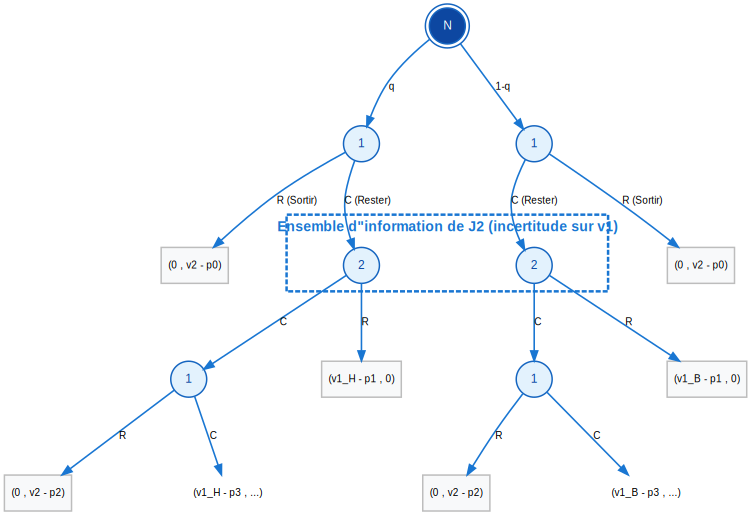
\includegraphics[width=25in]{auction_tree}

\begin{itemize}
\tightlist
\item
  Le nœud initial correspond au tirage du type de J1 par la Nature.
\item
  Les nœuds de décision représentent les choix successifs des joueurs aux différents niveaux de prix.
\item
  Les feuilles correspondent aux issues de l'enchère (retrait d'un joueur ou poursuite du processus).
\end{itemize}

À l'étape où le joueur 2 intervient, celui-ci ne connaît pas la valeur de \(v_1\).\\
Les nœuds correspondants sont donc regroupés dans un \textbf{ensemble d'information}, reflétant son incertitude sur le type de J1.

\begin{center}\rule{0.5\linewidth}{0.5pt}\end{center}

\section{Stratégies et croyances}\label{stratuxe9gies-et-croyances}

Une stratégie est un \textbf{plan contingent}, précisant pour chaque joueur :

\begin{itemize}
\tightlist
\item
  l'action à entreprendre à chaque nœud de décision,
\item
  conditionnellement à l'historique observé et, le cas échéant, à l'information privée.
\end{itemize}

Les croyances du joueur 2 portent sur la valeur de \(v_1\) et sont définies sur son ensemble d'information.\\
Elles sont notées :
\[
\mu_t = P(v_1 = v_{1H} \mid h_t),
\]
où \(h_t\) désigne l'historique observé à l'étape \(t\).

Ces croyances évoluent au cours de l'enchère, à mesure que les décisions observées restreignent l'ensemble des types possibles.

\begin{center}\rule{0.5\linewidth}{0.5pt}\end{center}

\section{Concept de solution}\label{concept-de-solution}

Le jeu ainsi défini est analysé à l'aide du concept d'\textbf{Équilibre Bayésien Parfait}.

Ce concept impose :

\begin{itemize}
\tightlist
\item
  que les stratégies soient \textbf{séquentiellement rationnelles} à chaque nœud du jeu ;
\item
  que les croyances soient \textbf{cohérentes} avec les stratégies et mises à jour conformément à la règle de Bayes.
\end{itemize}

La section suivante est consacrée à l'analyse de cet équilibre et à la caractérisation des comportements stratégiques qu'il induit.

\chapter{Equilibre parfait bayésien (EPB) dans l'enchère séquentielle}\label{equilibre-parfait-bayuxe9sien-epb-dans-lenchuxe8re-suxe9quentielle}

Cette partie présente le concept de solution utilisé pour analyser l'enchère séquentielle modélisée précédemment et explique comment l'équilibre est construit dans un jeu dynamique à information incomplète.

\section{Justification de la méthode}\label{justification-de-la-muxe9thode}

L'enchère considérée est un jeu dynamique, puisque les décisions des joueurs sont prises successivement, et à information incomplète, car les valeurs attribuées au bien sont privées. Elle est en outre informative, dans la mesure où les actions observées au cours de l'enchère (rester ou se retirer à un certain prix) modifient les croyances des joueurs sur les types de leurs adversaires. Dans un tel contexte, l'équilibre de Nash, conçu pour des jeux statiques, ainsi que l'équilibre de Nash bayésien, ne sont pas suffisants, car ils ne prennent pas en compte la chronologie des décisions et peuvent reposer sur des comportements non crédibles hors du chemin d'équilibre. Le concept de solution approprié est donc l'équilibre parfait bayésien, qui permet d'analyser simultanément la séquentialité des décisions et l'évolution des croyances.

\section{Définition opératoire de l'équilibre parfait bayésien}\label{duxe9finition-opuxe9ratoire-de-luxe9quilibre-parfait-bayuxe9sien}

L'analyse d'une enchère séquentielle à information incomplète requiert un concept d'équilibre qui tienne compte à la fois de la \textbf{chronologie des décisions} et de la \textbf{révision des croyances}.\\
Le concept pertinent est l'\textbf{équilibre parfait bayésien (EPB)}.

Un EPB est un couple \((\sigma, \mu)\), où :

\begin{itemize}
\item
  \(\sigma\) est un \textbf{profil de stratégies complètes}, spécifiant pour chaque joueur l'action à entreprendre à chaque nœud de décision, pour chaque type possible ;
\item
  \(\mu\) est un \textbf{système de croyances}, qui assigne, à chaque ensemble d'information, une probabilité aux différents types possibles des autres joueurs.
\end{itemize}

Le couple \((\sigma, \mu)\) constitue un équilibre parfait bayésien si et seulement si les deux conditions suivantes sont satisfaites.

\subsection{(i) Rationalité séquentielle}\label{i-rationalituxe9-suxe9quentielle}

À chaque étape de l'enchère, le joueur qui agit :

\begin{itemize}
\tightlist
\item
  connaît sa \textbf{valeur privée} ;
\item
  observe l'\textbf{historique du jeu} (prix atteints, retraits observés) ;
\item
  forme une \textbf{croyance} \(\mu\) sur le type de l'adversaire ;
\item
  choisit l'action (rester ou se retirer) qui \textbf{maximise son espérance de gain conditionnelle}.
\end{itemize}

Cette optimalité doit être vérifiée \textbf{à tous les nœuds du jeu}, y compris hors du chemin d'équilibre.\\
Elle exclut ainsi les \textbf{menaces non crédibles}, c'est-à-dire les comportements qui ne seraient pas rationnels s'ils devaient effectivement être mis en œuvre.

\subsection{(ii) Cohérence bayésienne et rôle informationnel des actions}\label{ii-cohuxe9rence-bayuxe9sienne-et-ruxf4le-informationnel-des-actions}

Les croyances ne sont pas arbitraires. Elles doivent être \textbf{cohérentes avec les stratégies} et mises à jour selon la \textbf{règle de Bayes}, partout où cela est possible.

Dans une enchère séquentielle, les actions observées jouent un rôle informationnel central :

\begin{itemize}
\item
  un \textbf{retrait} à un prix \(p\) implique que la valeur du joueur vérifie\\
  \[
  v_i \leq p ;
  \]
\item
  une \textbf{poursuite de l'enchère} à ce prix implique\\
  \[
  v_i \geq p .
  \]
\end{itemize}

À partir de ces observations, le joueur non informé révise ses croyances selon :
\[
\mu_{t+1} = P(v = v_H \mid \text{historique observé}).
\]

Les décisions prises au cours de l'enchère constituent ainsi des \textbf{signaux endogènes}, révélant progressivement de l'information sur les valeurs privées et guidant la dynamique stratégique.

\section{Signalisation, bluff et nature des équilibres}\label{signalisation-bluff-et-nature-des-uxe9quilibres}

Dans une enchère séquentielle, les actions des joueurs --- en particulier le fait de rester actif ou de se retirer à un certain niveau de prix --- ne sont pas de simples décisions mécaniques. Elles jouent un \textbf{rôle informationnel} : chaque action observée transmet un message sur la valeur privée du joueur qui agit.

Ce mécanisme relève de la \textbf{signalisation stratégique}. Une action constitue un signal crédible lorsqu'elle est \textbf{différentiellement coûteuse} selon le type du joueur. En particulier, poursuivre l'enchère à un prix élevé est relativement peu coûteux pour un joueur qui valorise fortement le bien, mais devient risqué, voire non rentable, pour un joueur de faible valorisation. C'est ce différentiel de coût qui permet aux actions de révéler de l'information.

Dans ce contexte, le \textbf{bluff} correspond au comportement d'un joueur de type faible qui imite la stratégie d'un type fort, en restant actif à des prix élevés, dans le but d'influencer les croyances de l'adversaire. L'objectif est de faire croire à une valorisation élevée afin de provoquer le retrait prématuré de l'autre joueur. Toutefois, le bluff n'est rationnel que si la probabilité de faire abandonner l'adversaire compense le risque de devoir acquérir le bien à un prix supérieur à sa propre valeur. Il s'agit donc d'un arbitrage stratégique entre gain informationnel et risque de surpaiement.

La manière dont la signalisation est exploitée par les joueurs détermine la \textbf{nature de l'équilibre parfait bayésien} observé.

\begin{itemize}
\item
  Dans un \textbf{équilibre séparateur}, chaque type de joueur adopte une stratégie distincte. Les actions observées permettent alors d'identifier parfaitement le type : après l'observation de l'action, les croyances a posteriori deviennent dégénérées, c'est-à-dire qu'un type est attribué avec probabilité un. L'asymétrie d'information disparaît et le jeu se transforme, à partir de ce point, en un jeu à information complète.
\item
  À l'inverse, dans un \textbf{équilibre mélangeant (ou pooling)}, plusieurs types choisissent volontairement la même stratégie. L'action observée ne permet plus de discriminer entre les types possibles. Les croyances a posteriori restent alors identiques aux croyances a priori, et l'incertitude persiste tout au long de l'enchère. Ce type d'équilibre est typiquement associé à des situations de bluff, où les types faibles parviennent à se rendre indiscernables des types forts.
\item
  Entre ces deux cas extrêmes existent des \textbf{équilibres semi-séparateurs}, dans lesquels certains types jouent des stratégies pures tandis que d'autres randomisent entre plusieurs actions. Ces équilibres intermédiaires sont fréquents dans les enchères séquentielles, car ils permettent de concilier incitations à révéler l'information et possibilités limitées de bluff.
\end{itemize}

\chapter{Exercice pratique}\label{exercice-pratique}

\section{Énoncé du problème}\label{uxe9noncuxe9-du-probluxe8me}

\textbf{Paramètres et information}

\begin{itemize}
\tightlist
\item
  Deux joueurs : J1 et J2\\
\item
  La Nature tire les valorisations privées\\
  \[
  v_1, v_2 \sim F
  \]
\item
  Chaque joueur connaît sa propre valeur mais ignore celle de l'autre\\
\item
  Le prix initial \(p\) est fixé par le commissaire-priseur\\
\item
  J2 observe l'action de J1 mais ne connaît pas \(v_1\)
\end{itemize}

\section{Déroulement du jeu et gains}\label{duxe9roulement-du-jeu-et-gains}

\textbf{Étape 1 -- Décision de J1}

J1 choisit :
- \textbf{R} : se retirer\\
- \textbf{C} : surenchérir à un prix \(p' > p\)

Si J1 choisit \textbf{R} :
- J2 gagne l'objet et paie \(p\)
- Gains :
\[
  u_1 = 0, \quad u_2 = v_2 - p
  \]

\begin{center}\rule{0.5\linewidth}{0.5pt}\end{center}

\textbf{Étape 2 -- Décision de J2 (si J1 a surenchéri)}

J2 choisit :
- \textbf{A} : accepter le prix \(p'\)
- \textbf{R} : refuser

Si J2 \textbf{accepte (A)} :
- J2 gagne et paie \(p'\)
- Gains :
\[
  u_1 = 0, \quad u_2 = v_2 - p'
  \]

Si J2 \textbf{refuse (R)} :
- J1 gagne et paie \(p'\)
- Gains :
\[
  u_1 = v_1 - p', \quad u_2 = 0
  \]

\begin{center}\rule{0.5\linewidth}{0.5pt}\end{center}

\section{Arbre du jeu}\label{arbre-du-jeu}

\begin{figure}
\centering
\includegraphics{images/image.png}
\caption{Arbre du jeu}
\end{figure}

\section{RÉSOLUTION (INDUCTION RÉTROGRADE)}\label{ruxe9solution-induction-ruxe9trograde}

Dans un jeu séquentiel à information incomplète, nous résolvons en partant de la dernière étape pour assurer la \textbf{perfection en sous-jeux}.

\begin{center}\rule{0.5\linewidth}{0.5pt}\end{center}

\subsection{Étape 1 : Décision optimale du Joueur 2}\label{uxe9tape-1-duxe9cision-optimale-du-joueur-2}

Le Joueur 2 (J2) observe le prix \(p'\) proposé par J1. Il connaît sa propre valeur \(v_2\), mais ignore la valeur \(v_1\).

Soit \(\mu = \mathbb{P}(v_1 | p')\) la croyance de J2 sur le type de J1 après observation de la surenchère.

\subsubsection{Espérance d'utilité de J2}\label{espuxe9rance-dutilituxe9-de-j2}

\begin{enumerate}
\def\labelenumi{\arabic{enumi}.}
\tightlist
\item
  \textbf{S'il accepte (A)} : J2 obtient l'objet avec certitude au prix \(p'\).
  \[\mathbb{E}[u_2(A)] = v_2 - p'\]
\item
  \textbf{S'il refuse (R)} : J2 n'obtient pas l'objet et ne paie rien.
  \[\mathbb{E}[u_2(R)] = 0\]
\end{enumerate}

\subsubsection{Condition de décision}\label{condition-de-duxe9cision}

J2 accepte si et seulement si :
\[\mathbb{E}[u_2(A)] \geq \mathbb{E}[u_2(R)] \implies v_2 - p' \geq 0\]

\begin{quote}
** Stratégie optimale de J2** :
\[\boxed{s_2^*(p', v_2) = \text{Accepter si } p' \leq v_2}\]

\emph{Note: Cette décision est une \textbf{stratégie dominante} au stade de la sous-enchère ; elle ne dépend pas de la croyance \(\mu\) car le gain de J2 est indépendant du type de J1 une fois le prix \(p'\) fixé.}
\end{quote}

\subsection{Étape 2 : Anticipation du Joueur 1}\label{uxe9tape-2-anticipation-du-joueur-1}

Le Joueur 1 (J1) anticipe la réponse de J2. Il sait que :
* Si \(p' \leq v_2\), J2 accepte \(\implies\) J1 perd (utilité \(0\)).
* Si \(p' > v_2\), J2 refuse \(\implies\) J1 gagne au prix \(p'\) (utilité \(v_1 - p'\)).

Comme J1 ne connaît pas \(v_2\), il utilise la fonction de répartition \(F\) pour évaluer la probabilité que J2 refuse :
\[\mathbb{P}(\text{J2 refuse}) = \mathbb{P}(v_2 < p') = F(p')\]

\subsubsection{Espérance d'utilité de J1}\label{espuxe9rance-dutilituxe9-de-j1}

\[EU_1(p' | v_1) = F(p') \cdot (v_1 - p') + (1 - F(p')) \cdot 0\]
\[EU_1(p' | v_1) = F(p') \cdot (v_1 - p')\]

J1 choisit de surenchérir à \(p'\) plutôt que de se retirer à \(p\) si et seulement si :
\[EU_1(p' | v_1) \geq 0 \implies v_1 \geq p'\]

\subsection{Étape 3 : Équilibre Parfait Bayésien (EPB)}\label{uxe9tape-3-uxe9quilibre-parfait-bayuxe9sien-epb}

Un \textbf{Équilibre Parfait Bayésien} est un triplet (stratégies, croyances, rationalité) tel que :

\begin{enumerate}
\def\labelenumi{\arabic{enumi}.}
\tightlist
\item
  \textbf{Rationalité séquentielle} : J2 suit sa stratégie dominante \(v_2 \geq p'\).
\item
  \textbf{Action de J1} : J1 propose \(p'\) si \(v_1\) est suffisamment élevé pour que \(EU_1(p') > 0\).
\item
  \textbf{Coyances cohérentes} : J2 maintient des croyances \(\mu\) compatibles avec la stratégie de J1 (bien qu'ici, l'action de J2 soit indépendante de ces croyances).
\end{enumerate}

\subsection{CONCLUSION}\label{conclusion}

Dans cette enchère séquentielle :
* Le joueur qui décide en dernier (J2) suit une règle de \textbf{valeur intrinsèque} : il accepte si le prix est inférieur à sa valeur privée, \textbf{indépendamment} de ses croyances sur l'autre joueur.
* Le premier joueur (J1) fait face à un arbitrage entre la probabilité de gagner (qui augmente avec \(p'\)) et la marge bénéficiaire \((v_1 - p')\).

\begin{quote}
\textbf{Résultat remarquable} : Contrairement à d'autres jeux de signalisation, l'asymétrie d'information n'altère pas la décision finale de J2, mais elle conditionne la prise de risque initiale de J1.
\end{quote}

\chapter{Prolongement pour plusieurs biens}\label{prolongement-pour-plusieurs-biens}

Lorsque plusieurs biens sont vendus successivement, l'enchère ne peut plus être analysée comme une simple répétition d'enchères indépendantes.\\
La \textbf{dimension temporelle} modifie profondément les incitations des enchérisseurs : chaque décision affecte non seulement l'allocation courante, mais aussi les opportunités futures.

Cette section met en évidence les principaux mécanismes stratégiques qui émergent spécifiquement dans les enchères séquentielles multi-biens.

\begin{center}\rule{0.5\linewidth}{0.5pt}\end{center}

\section{Valeur d'option et arbitrage intertemporel}\label{valeur-doption-et-arbitrage-intertemporel}

Dans une enchère séquentielle, gagner un bien à une date donnée empêche de participer aux enchères ultérieures pour des biens potentiellement substituables.\\
Cette contrainte introduit une \textbf{valeur d'option} associée à l'attente.

Un enchérisseur rationnel ne compare donc pas uniquement sa valorisation actuelle \(v_i\) au prix courant, mais intègre également la valeur espérée des opportunités futures.\\
Son enchère effective au tour \(t\) reflète ainsi un arbitrage intertemporel de la forme :
\[
\text{disposition à payer} = v_i^{(t)} - \mathbb{E}[\text{gain futur}],
\]
où l'espérance porte sur les enchères à venir.

Cette logique explique une \textbf{retenue stratégique} précoce, même pour des enchérisseurs ayant une valorisation élevée du bien courant.

\begin{center}\rule{0.5\linewidth}{0.5pt}\end{center}

\section{Effet de remplacement et dynamique de la demande}\label{effet-de-remplacement-et-dynamique-de-la-demande}

Lorsque les biens vendus sont \textbf{substituables}, l'obtention d'un bien réduit l'utilité marginale des suivants.\\
C'est le \textbf{remplacement inter-biens}.

\begin{itemize}
\tightlist
\item
  Après avoir remporté un premier lot, un enchérisseur ajuste à la baisse son agressivité sur les lots suivants.
\item
  À l'inverse, un enchérisseur ayant perdu un lot peut devenir plus agressif par nécessité de compensation.
\end{itemize}

La demande n'est donc ni fixe ni indépendante : elle évolue endogènement au fil des adjudications.\\
Cette dynamique explique pourquoi les équilibres observés dans les enchères séquentielles diffèrent fondamentalement de ceux des enchères simultanées.

\begin{center}\rule{0.5\linewidth}{0.5pt}\end{center}

\section{Révélation progressive de l'information}\label{ruxe9vuxe9lation-progressive-de-linformation}

Les enchères séquentielles génèrent un \textbf{processus endogène d'apprentissage}.

À chaque tour, le prix d'adjudication et l'identité du gagnant deviennent des informations publiques.\\
Les enchérisseurs restants utilisent ces observations pour mettre à jour leurs croyances sur :

\begin{itemize}
\tightlist
\item
  les valorisations privées,
\item
  la capacité financière,
\item
  ou l'intensité concurrentielle des autres participants.
\end{itemize}

Cette mise à jour s'effectue selon la \textbf{règle de Bayes}, transformant progressivement l'environnement stratégique.

\subsection{Principe de liaison (Milgrom \& Weber, 1982)}\label{principe-de-liaison-milgrom-weber-1982}

Lorsque les actions révèlent de l'information pertinente, la transparence tend à :

\begin{itemize}
\tightlist
\item
  réduire l'incertitude,
\item
  accroître l'agressivité des enchères,
\item
  augmenter le revenu espéré du vendeur.
\end{itemize}

Ce mécanisme explique pourquoi les enchères ouvertes et séquentielles peuvent dominer les formats scellés dans certains contextes.

\begin{center}\rule{0.5\linewidth}{0.5pt}\end{center}

\section{Signalisation, intimidation et comportements stratégiques}\label{signalisation-intimidation-et-comportements-stratuxe9giques}

La répétition des interactions permet l'émergence de stratégies de \textbf{signalisation}.

\subsection{Jump bidding}\label{jump-bidding}

Un enchérisseur peut soumettre volontairement une enchère très supérieure au minimum requis afin de :

\begin{itemize}
\tightlist
\item
  signaler une valorisation élevée,
\item
  décourager les concurrents,
\item
  raccourcir la durée de l'enchère.
\end{itemize}

Ce comportement peut être rationnel s'il réduit la concurrence future à un coût acceptable.

\subsection{Stratégies de prédation}\label{stratuxe9gies-de-pruxe9dation}

Dans certains contextes, un acteur dominant peut accepter de \textbf{surpayer un premier bien} pour provoquer la sortie de concurrents plus faibles.\\
Le surpaiement initial devient alors un investissement stratégique visant à améliorer la position concurrentielle sur les enchères suivantes.

\begin{center}\rule{0.5\linewidth}{0.5pt}\end{center}

\section{Malédiction du vainqueur et effets dynamiques}\label{maluxe9diction-du-vainqueur-et-effets-dynamiques}

Dans les enchères à \textbf{valeurs communes}, la séquentialité amplifie la malédiction du vainqueur.

\begin{itemize}
\tightlist
\item
  Remporter un premier bien révèle une estimation relativement optimiste.
\item
  Ex post, le gagnant infère que les autres enchérisseurs avaient des évaluations plus faibles.
\item
  Les enchères ultérieures sont alors abordées avec davantage de prudence.
\end{itemize}

Cette dynamique peut conduire à une baisse progressive des prix, même pour des biens identiques.

\begin{center}\rule{0.5\linewidth}{0.5pt}\end{center}

\section{Baisse des prix et paradoxe de l'enchère déclinante}\label{baisse-des-prix-et-paradoxe-de-lenchuxe8re-duxe9clinante}

Empiriquement, on observe fréquemment que des biens identiques vendus successivement le sont à des prix décroissants, phénomène parfois appelé \emph{afternoon effect}.

Plusieurs mécanismes contribuent à ce résultat :

\begin{itemize}
\tightlist
\item
  \textbf{Diminution de la concurrence} : chaque adjudication élimine un enchérisseur potentiel.
\item
  \textbf{Aversion au risque} : certains acheteurs acceptent de payer plus tôt pour éviter l'incertitude.
\item
  \textbf{Fatigue stratégique} : la durée et le coût cognitif de la participation réduisent l'agressivité des offres.
\end{itemize}

Ce paradoxe souligne que les prix séquentiels reflètent autant la structure stratégique que les caractéristiques intrinsèques des biens.

Les enchères séquentielles à plusieurs biens mettent en évidence que :
- les décisions sont fondamentalement intertemporelles,
- l'information est révélée de manière progressive,
- les stratégies combinent arbitrage, signalisation et anticipation.

\chapter{Conclusion}\label{conclusion-1}

Ce travail a analysé les enchères séquentielles à l'aide du cadre des jeux dynamiques à information incomplète.\\
L'objectif était de montrer que la séquentialité constitue une dimension stratégique centrale qui modifie à la fois les comportements, l'information et les résultats d'allocation.

Dans le cas d'un bien unique, l'enchère séquentielle se caractérise par :

\begin{itemize}
\tightlist
\item
  une chronologie explicite des décisions,
\item
  une information initialement incomplète liée aux valeurs privées,
\item
  et une révélation progressive de l'information à travers les actions observées.
\end{itemize}

Ces caractéristiques rendent inadaptés les concepts d'équilibre statiques.\\
L'équilibre parfait bayésien fournit alors un cadre de résolution cohérent, en imposant simultanément :

\begin{itemize}
\tightlist
\item
  la rationalité séquentielle à chaque étape du jeu,
\item
  et la cohérence des croyances via la règle de Bayes.
\end{itemize}

L'extension au cas de plusieurs biens met en évidence des mécanismes spécifiquement dynamiques.\\
La valeur d'option associée aux tours futurs, l'effet de remplacement entre biens, ainsi que la révélation endogène de l'information modifient les incitations individuelles et expliquent des régularités empiriques observées, telles que la baisse progressive des prix ou les stratégies d'intimidation.

Dans l'ensemble, l'analyse montre que les enchères séquentielles constituent des dispositifs où décisions, information et anticipations évoluent conjointement.\\
Elles justifient pleinement l'usage des outils de la théorie des jeux dynamiques bayésiens.

Malgré sa cohérence interne, le cadre théorique retenu repose sur plusieurs hypothèses restrictives.

\section{Hypothèse de rationalité parfaite}\label{hypothuxe8se-de-rationalituxe9-parfaite}

Le modèle suppose que les enchérisseurs :

\begin{itemize}
\tightlist
\item
  sont parfaitement rationnels,
\item
  anticipent correctement les comportements futurs,
\item
  et mettent à jour leurs croyances conformément à la règle de Bayes.
\end{itemize}

En pratique, des limites cognitives ou des heuristiques peuvent conduire à des écarts systématiques par rapport aux prédictions théoriques.

\section{Absence de contraintes budgétaires explicites}\label{absence-de-contraintes-budguxe9taires-explicites}

Les modèles standards abstraient généralement des contraintes de liquidité.\\
Or, dans de nombreuses enchères réelles, les budgets limités, les coûts de financement ou les restrictions institutionnelles influencent fortement les stratégies.

\section{Structure simplifiée de l'information}\label{structure-simplifiuxe9e-de-linformation}

L'analyse repose sur :
- un nombre fini de types,
- des distributions communes connues,
- et une observation parfaite des actions passées.

Dans les contextes réels, l'information peut être bruitée, partielle ou imparfaitement observée, ce qui complique la formation et la mise à jour des croyances.

\section{Absence de comportements collusifs et de règles institutionnelles}\label{absence-de-comportements-collusifs-et-de-ruxe8gles-institutionnelles}

Le cadre est non coopératif et ne prend pas en compte :

\begin{itemize}
\tightlist
\item
  les accords explicites ou tacites entre enchérisseurs,
\item
  ni les règles spécifiques de conception des mécanismes d'enchères.
\end{itemize}

Ces éléments peuvent modifier substantiellement les résultats théoriques.

\section{Portée empirique}\label{portuxe9e-empirique}

Enfin, les résultats dépendent étroitement des hypothèses retenues (valeurs privées ou communes, substituabilité des biens, ordre de vente).\\
Leur validité empirique doit être évaluée au cas par cas à l'aide de données ou d'analyses expérimentales.

Ces limites suggèrent plusieurs prolongements:

\begin{itemize}
\tightlist
\item
  l'introduction de contraintes budgétaires et de rationalité limitée,
\item
  l'étude d'enchères combinatoires ou hybrides,
\item
  et l'analyse empirique des enchères séquentielles observées sur les marchés réels.
\end{itemize}

Elles soulignent que, si le cadre théorique est robuste, son enrichissement est nécessaire pour mieux rendre compte de la complexité des environnements concrets.

\end{document}
